\documentclass[xetex,mathserif,serif]{beamer}
\usepackage{polyglossia}
\setdefaultlanguage[babelshorthands=true]{russian}
\usepackage{minted}
\usepackage{tabu}

\useoutertheme{infolines}

\usepackage{fontspec}
\setmainfont{FreeSans}
\newfontfamily{\russianfonttt}{FreeSans}

\tabulinesep=0.7mm

\newcommand{\attribution}[1] {
	\vspace{-5mm}\begin{flushright}\begin{scriptsize}\textcolor{gray}{\textcopyright\, #1}\end{scriptsize}\end{flushright}
}

\title{Лекция 10: Архитектурные стили}
\author[Юрий Литвинов]{Юрий Литвинов \newline \textcolor{gray}{\small\texttt{yurii.litvinov@gmail.com}}}

\date{03.11.2020г}

\begin{document}
	
	\frame{\titlepage}

	\section{Введение}

	\begin{frame}
		\frametitle{Архитектурные шаблоны и стили}
		Архитектурный стиль --- набор решений, которые
		\begin{enumerate}
			\item применимы в выбранном контексте разработки,
			\item задают ограничения на принимаемые архитектурные решения, специфичные для определённых систем в этом контексте,
			\item приводят к желаемым положительным качествам получаемой системы.
		\end{enumerate}
		Архитектурный шаблон --- именованный набор ключевых проектных решений по эффективной организации подсистем, применимых для повторяемых технических задач проектирования в различных контекстах и предметных областях
	\end{frame}

	\begin{frame}
		\frametitle{Архитектурные шаблоны и стили, классификация}
		\begin{center}
			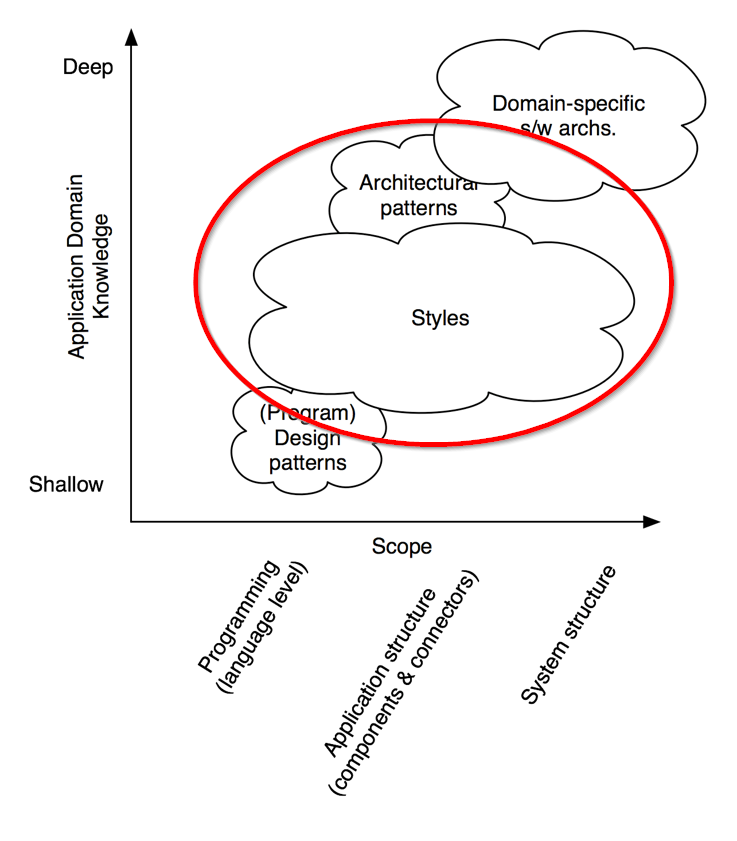
\includegraphics[width=0.5\textwidth]{architecturalStylesHighlighted.png}
			\attribution{N. Medvidovic}
		\end{center}
	\end{frame}

	\section{Примеры архитектурных шаблонов}

	\begin{frame}
		\frametitle{Пример: трёхзвенная архитектура}
		\framesubtitle{State-Logic-Display}
		\begin{columns}
			\begin{column}{0.5\textwidth}
				Примеры применения
				\begin{itemize}
					\item Бинес-приложения
					\item Многопользовательские игры
					\item Веб-приложения
				\end{itemize}
			\end{column}
			\begin{column}{0.5\textwidth}
				\begin{center}
					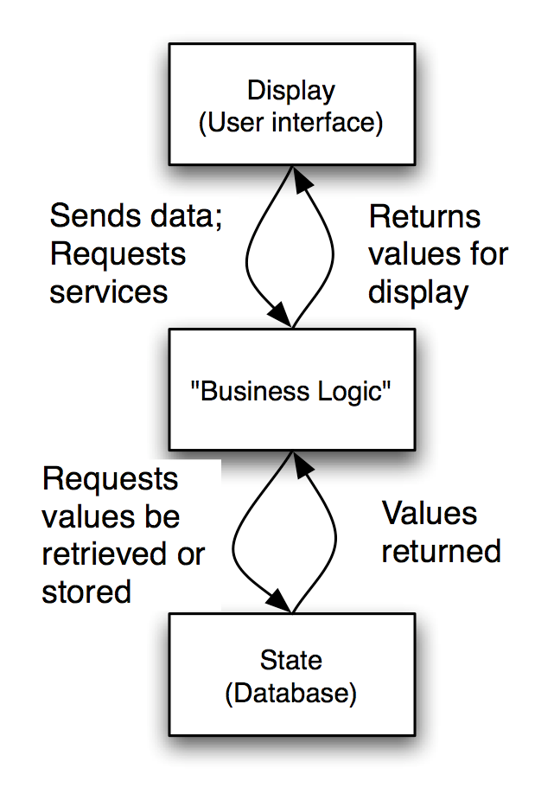
\includegraphics[width=0.7\textwidth]{threeTieredArchitecture.png}
					\attribution{N. Medvidovic}
				\end{center}
			\end{column}
		\end{columns}
	\end{frame}

	\begin{frame}
		\frametitle{Пример: Model-View-Controller}
		\begin{center}
			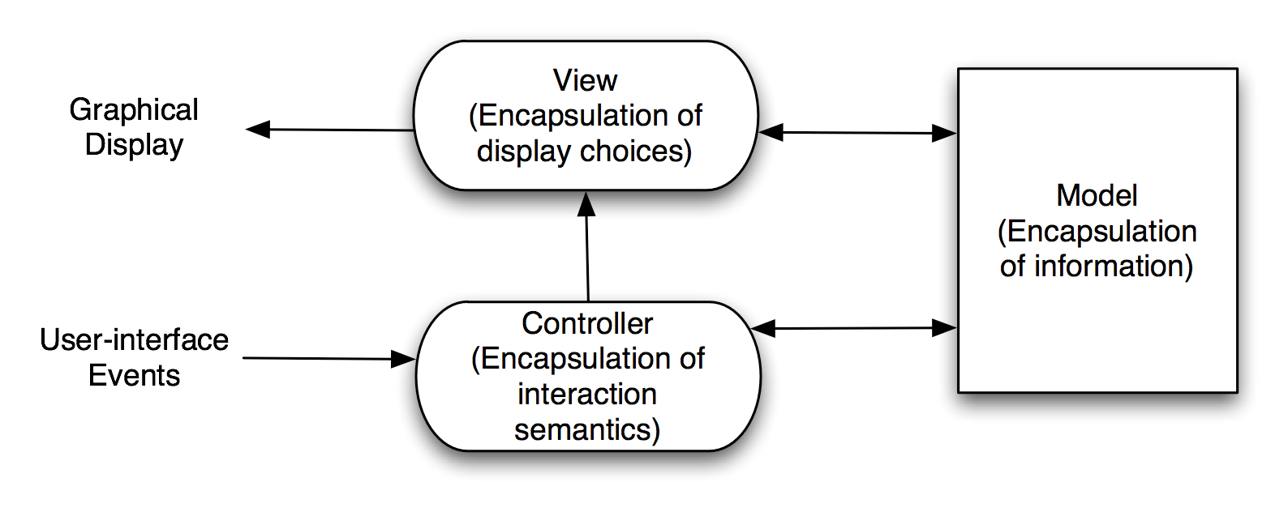
\includegraphics[width=0.65\textwidth]{mvc.png}
			\attribution{N. Medvidovic}
		\end{center}
		\begin{itemize}
			\item Разделяет данные, представление и взаимодействие с пользователем
			\item Если в модели что-то меняется, она оповещает представление (представления)
			\item Через контроллер проходит всё взаимодействие с пользователем
			\begin{itemize}
				\item Естественное место для паттерна ``Команда'' и Undo/Redo
			\end{itemize}
		\end{itemize}
	\end{frame}

	\begin{frame}
		\frametitle{Пример: Sense-Compute-Control}
		\begin{center}
			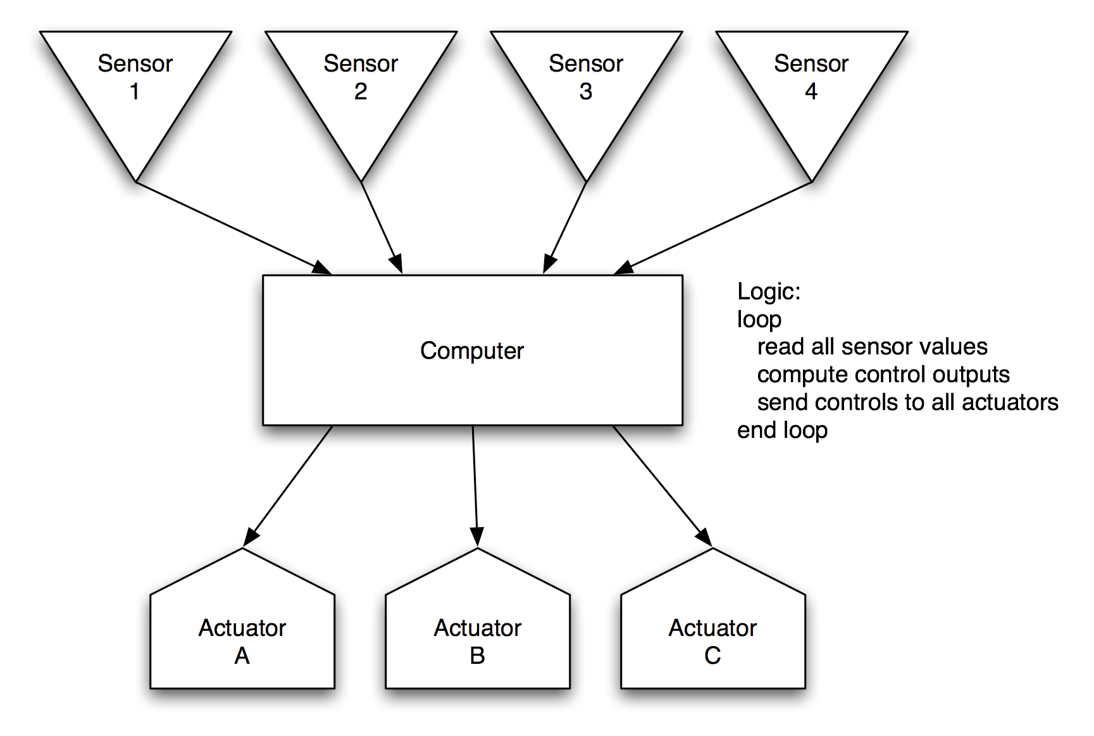
\includegraphics[width=0.65\textwidth]{senseComputeControl.png}
			\attribution{N. Medvidovic}
		\end{center}
		\begin{itemize}
			\item Применяется во встроенных системах и робототехнике
		\end{itemize}
	\end{frame}

	\section{Архитектурные стили}

	\begin{frame}
		\frametitle{Архитектурные стили}
		\begin{itemize}
			\item Именованная коллекция архитектурных решений
			\item Менее узкоспециализированные, чем архитектурные паттерны
		\end{itemize}
		\begin{center}
			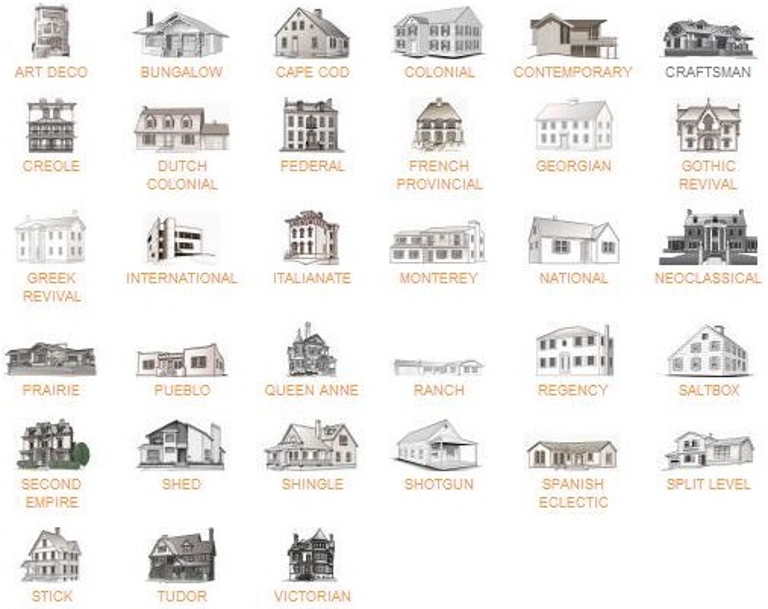
\includegraphics[width=0.5\textwidth]{buildingStyles.png}
			\attribution{N. Medvidovic}
		\end{center}
	\end{frame}

	\begin{frame}
		\frametitle{Архитектурные стили}
		\begin{columns}
			\begin{column}{0.5\textwidth}
				\begin{itemize}
					\item Одна система может включать в себя несколько архитектурных стилей
					\item Понятие стиля применимо и к подсистемам
				\end{itemize}
			\end{column}
			\begin{column}{0.5\textwidth}
				\begin{center}
					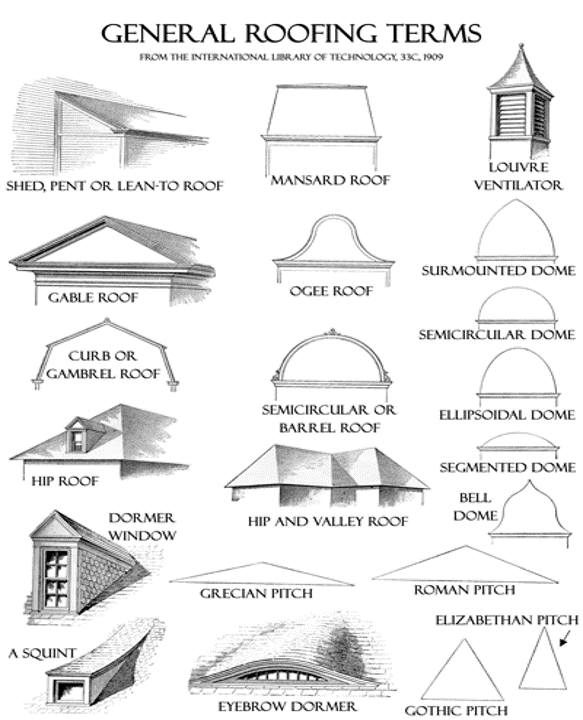
\includegraphics[width=0.7\textwidth]{roofStyles.png}
					\attribution{N. Medvidovic}
				\end{center}
			\end{column}
		\end{columns}
	\end{frame}

	\begin{frame}
		\frametitle{Преимущества использования стилей}
		\begin{itemize}
			\item Переиспользование архитектуры
			\begin{itemize}
				\item Для новых задач можно применять хорошо известные и изученные решения
			\end{itemize}
			\item Переиспользование кода
			\begin{itemize}
				\item Часто у стилей бывают неизменяемые части, которые можно один раз реализовать
			\end{itemize}
			\item Упрощение общения и понимания системы
			\item Упрощение интеграции приложений
			\item Специфичные для стиля методы анализа
			\begin{itemize}
				\item Возможны благодаря ограничениям на структуру системы
			\end{itemize}
			\item Специфичные для стиля методы визуализации
		\end{itemize}
	\end{frame}

	\begin{frame}
		\frametitle{Основные характеристики стилей}
		\begin{itemize}
			\item Набор используемых элементов архитектуры
			\begin{itemize}
				\item Типы компонентов и соединителей, элементы данных
				\begin{itemize}
					\item Например, объекты, фильтры, сервера и т.д.
				\end{itemize}
			\end{itemize}
			\item Набор правил конфигурирования
			\begin{itemize}
				\item ``Топологические'' ограничения на соединение элементов
				\begin{itemize}
					\item Например, компонент может быть соединён с максимум двумя компонентами
				\end{itemize}
			\end{itemize}
			\item Семантика, стоящая за элементами
		\end{itemize}
	\end{frame}

	\section{Lunar lander}

	\begin{frame}
		\frametitle{Игра ``Посадка на луну''}
		\framesubtitle{Lunar Lander}
		\begin{columns}
			\begin{column}{0.5\textwidth}
				\begin{itemize}
					\item Игрок управляет двигателем спускаемого аппарата
					\item Топливо ограничено
					\item Заданы начальная высота и скорость
					\item Победа засчитывается, если скорость при касании грунта меньше заданной
					\item Продвинутая версия позволяет управлять горизонтальным движением
				\end{itemize}
			\end{column}
			\begin{column}{0.5\textwidth}
				\begin{center}
					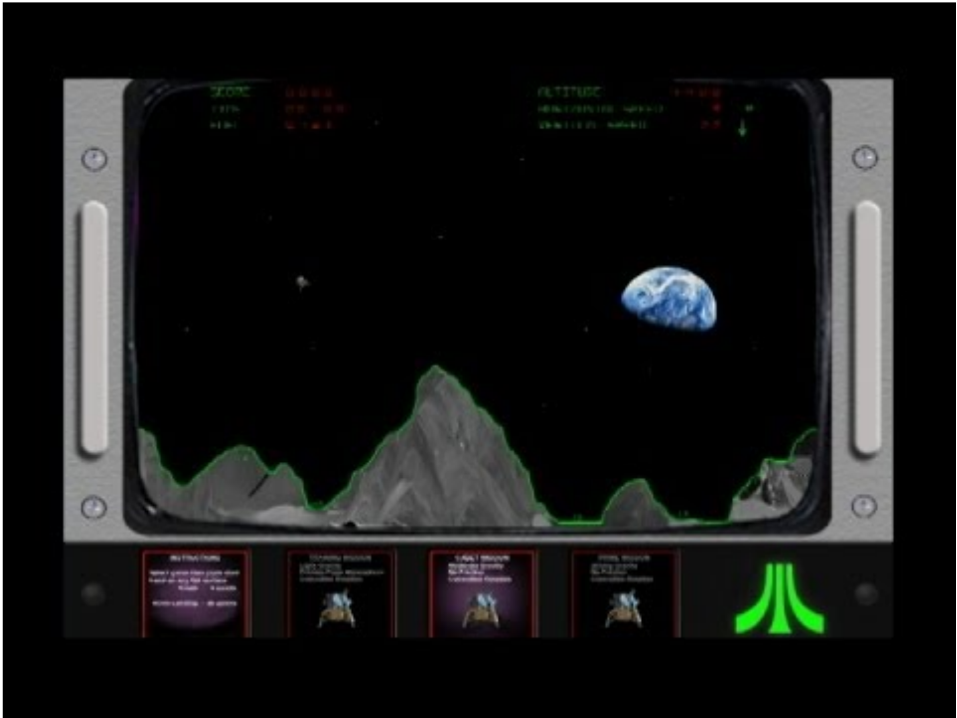
\includegraphics[width=0.9\textwidth]{lunarLander.png}
					\attribution{N. Medvidovic}
				\end{center}
			\end{column}
		\end{columns}
	\end{frame}

	\begin{frame}
		\frametitle{Sense-Compute-Control-реализация}
		\begin{center}
			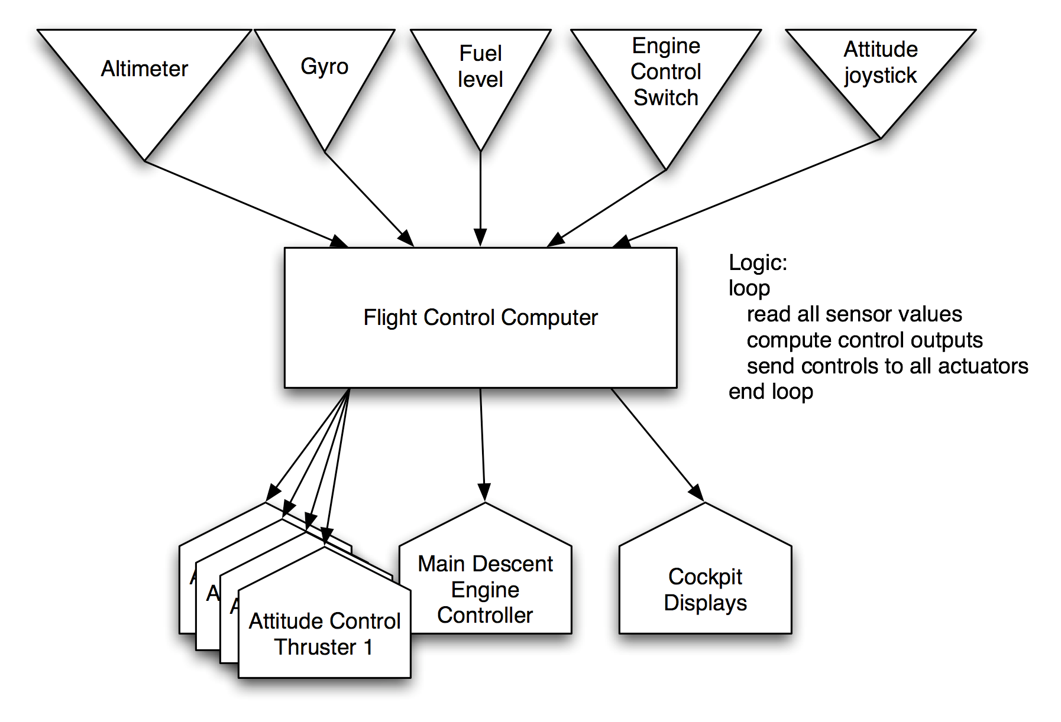
\includegraphics[width=0.7\textwidth]{senseComputeControlLunarLander.png}
			\attribution{N. Medvidovic}
		\end{center}
	\end{frame}

	\section{Архитектурные стили}

	\begin{frame}
		\frametitle{Некоторые известные стили}
		\begin{columns}
			\begin{column}{0.5\textwidth}
				\begin{itemize}
					\item ``Традиционные'', связанные с языком
					\begin{itemize}
						\item Главная программа/подпрограммы
						\item Объектно-ориентированный
					\end{itemize}
					\item Уровневый стиль
					\begin{itemize}
						\item Виртуальные машины
						\item Клиент-сервер
					\end{itemize}
					\item Стили, ориентированные на поток данных
					\begin{itemize}
						\item Пакетное исполнение
						\item Каналы и фильтры
					\end{itemize}
					\item Peer-to-peer
				\end{itemize}
			\end{column}
			\begin{column}{0.5\textwidth}
				\begin{itemize}
					\item Общая память
					\begin{itemize}
						\item Blackboard
						\item Ориентированные на правила
					\end{itemize}
					\item Интерпретаторы
					\begin{itemize}
						\item Интерпретатор
						\item Мобильный код
					\end{itemize}
					\item Неявный вызов
					\begin{itemize}
						\item Событийно-ориентированный
						\item Издатель-подписчик
					\end{itemize}
					\item ``Производные'' стили
					\begin{itemize}
						\item Распределённые объекты
						\item REST
						\item C2
					\end{itemize}
				\end{itemize}
			\end{column}
		\end{columns}
	\end{frame}

	\section{Главная программа и подпрограммы}

	\begin{frame}
		\frametitle{Главная программа/подпрограммы}
		\begin{center}
			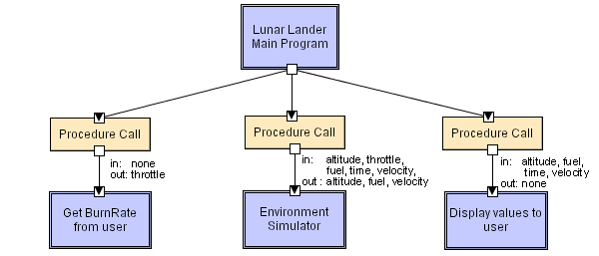
\includegraphics[width=0.8\textwidth]{mainProgramAndSubroutinesLL.png}
			\attribution{N. Medvidovic}
		\end{center}
	\end{frame}

	\section{Объектно-ориентированный стиль}

	\begin{frame}
		\frametitle{Объектно-ориентированный стиль}
		\begin{itemize}
			\item Компоненты --- объекты
			\item Соединители --- сообщения и вызовы методов
			\item Инварианты:
			\begin{itemize}
				\item Объекты отвечают за своё внутреннее состояние
				\item Реализация скрыта от других объектов
			\end{itemize}
			\item Преимущества:
			\begin{itemize}
				\item Декомпозиция системы в набор взаимодействующих агентов
				\item Внутреннее представление объектов можно менять независимо
				\item Близко к предметной области
			\end{itemize}
			\item Недостатки:
			\begin{itemize}
				\item Побочные эффекты при вызове методов
				\item Объекты вынуждены знать обо всех, от кого зависят
			\end{itemize}
		\end{itemize}
	\end{frame}

	\begin{frame}
		\frametitle{Объектно-ориентированный стиль, Lunar Lander}
		\begin{center}
			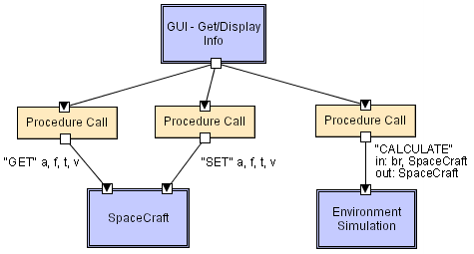
\includegraphics[width=0.7\textwidth]{objectOrientedLL.png}
			\attribution{N. Medvidovic}
		\end{center}
	\end{frame}

	\begin{frame}
		\frametitle{Или то же на UML}
		\begin{center}
			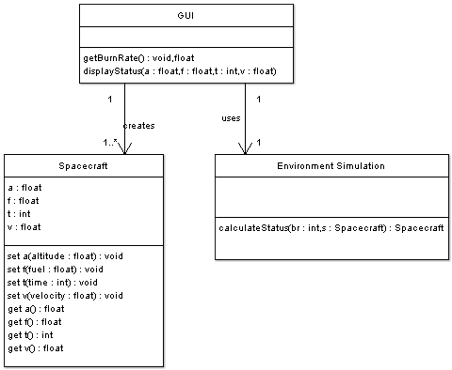
\includegraphics[width=0.5\textwidth]{objectOrientedLLUML.png}
			\attribution{N. Medvidovic}
		\end{center}
	\end{frame}

	\section{Слоистый стиль}

	\begin{frame}
		\frametitle{Слоистый стиль}
		\framesubtitle{Layered style}
		\begin{columns}
			\begin{column}{0.85\textwidth}
				\begin{itemize}
					\item Иерархическая организация системы
					\begin{itemize}
						\item ``Многоуровневый клиент-сервер''
						\item Каждый слой предоставляет интерфейс для использования слоями выше
					\end{itemize}
					\item Каждый слой работает как:
					\begin{itemize}
						\item Сервер --- предоставляет функциональность слоям выше
						\item Клиент --- использует функциональность слоёв ниже
					\end{itemize}
					\item Соединители --- протоколы взаимодействия слоёв
					\item Пример --- операционные системы, сетевые стеки протоколов
				\end{itemize}
			\end{column}
			\begin{column}{0.19\textwidth}
				\begin{center}
					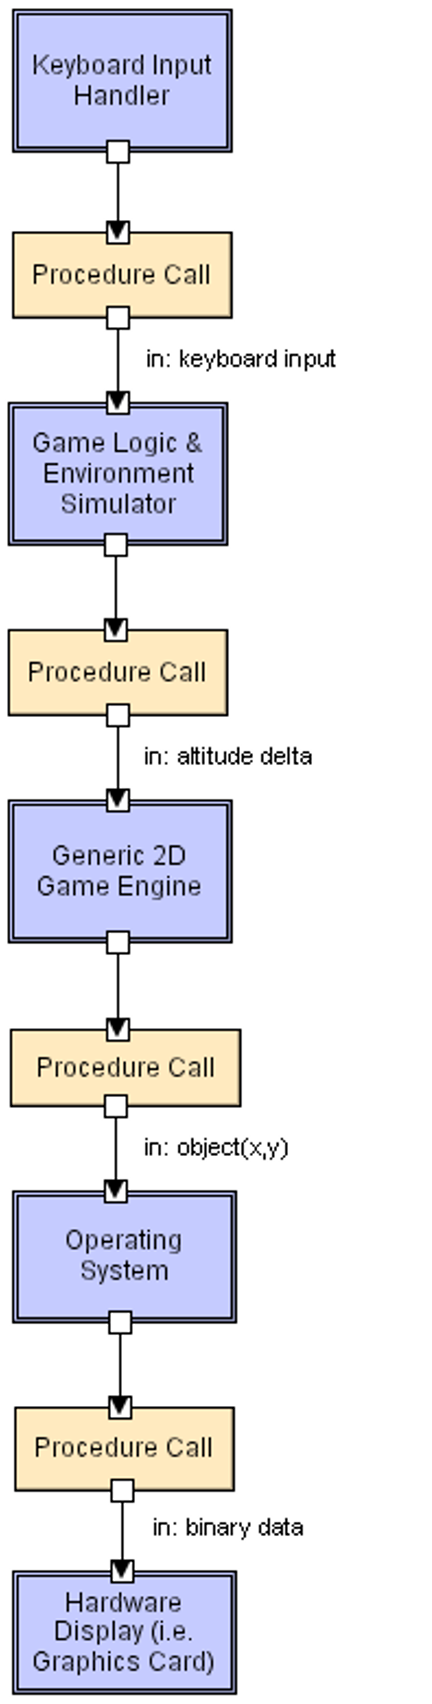
\includegraphics[width=0.8\textwidth]{layeredLL.png}
				\end{center}
			\end{column}
		\end{columns}
	\end{frame}

	\begin{frame}
		\frametitle{Слоистый стиль, подробности}
		\begin{columns}
			\begin{column}{0.5\textwidth}
				\begin{itemize}
					\item Преимущества:
					\begin{itemize}
						\item Повышение уровня абстракции
						\item Лёгкость в расширении
						\item Изменения в каждом уровне затрагивают максимум два соседних
						\item Возможны разные реализации уровня, если они удовлетворяют интерфейсу
					\end{itemize}
					\item Недостатки:
					\begin{itemize}
						\item Не всегда применим
						\item Проблемы с производительностью
					\end{itemize}
				\end{itemize}
			\end{column}
			\begin{column}{0.5\textwidth}
				\begin{center}
					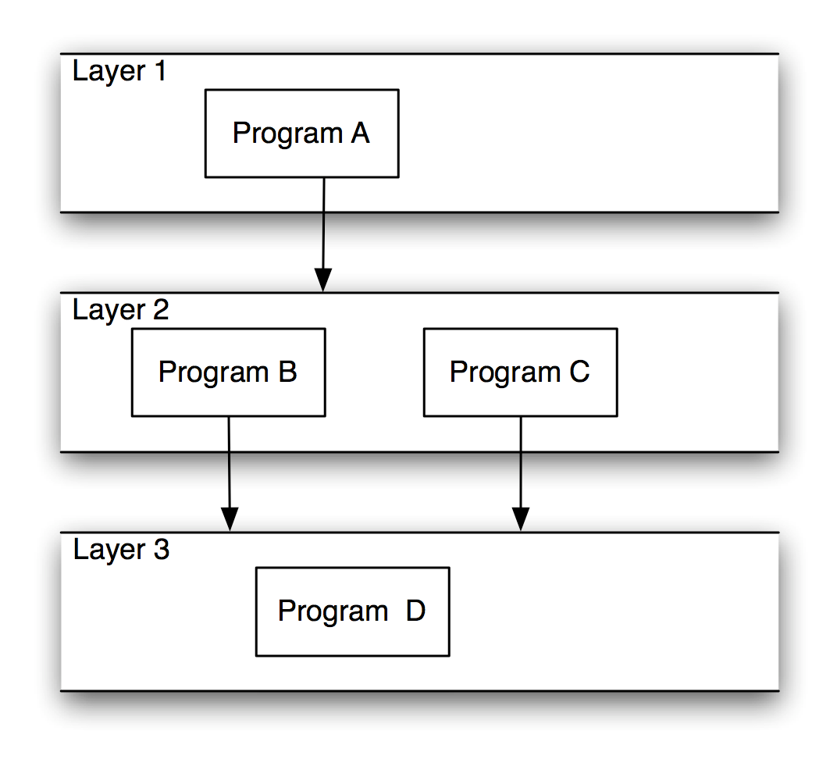
\includegraphics[width=0.8\textwidth]{layered.png}
					\attribution{N. Medvidovic}
				\end{center}
			\end{column}
		\end{columns}
	\end{frame}

	\section{Клиент-сервер}

	\begin{frame}
		\frametitle{``Клиент-сервер''}
		\begin{itemize}
			\item Компоненты --- клиенты и серверы
			\item Серверы не знают ничего о клиентах, даже их количество
			\item Клиенты знают только про сервера и не могут общаться друг с другом
			\item Соединители --- сетевые протоколы
		\end{itemize}
	\end{frame}

	\begin{frame}
		\frametitle{``Клиент-сервер'', Lunar Lander}
		\begin{center}
			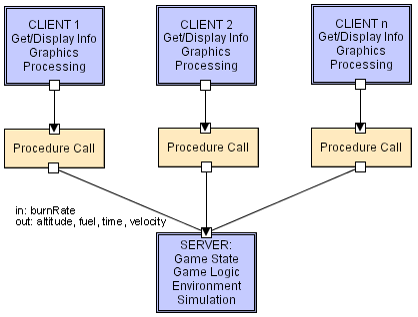
\includegraphics[width=0.6\textwidth]{clientServerLL.png}
			\attribution{N. Medvidovic}
		\end{center}
	\end{frame}

	\section{Пакетная обработка}

	\begin{frame}
		\frametitle{Пакетная обработка}
		\begin{itemize}
			\item Система строится как набор отдельных программ, выполняющихся последовательно
			\item Данные стандартным для ОС способом передаются от программы к программе
			\begin{itemize}
				\item Pipes, named pipes, файлы
			\end{itemize}
			\item Данные --- в явном виде всё, необходимое для работы
		\end{itemize}
		Типичен для финансовых систем глубокой древности (``Прадедушка стилей'')
		\begin{center}
			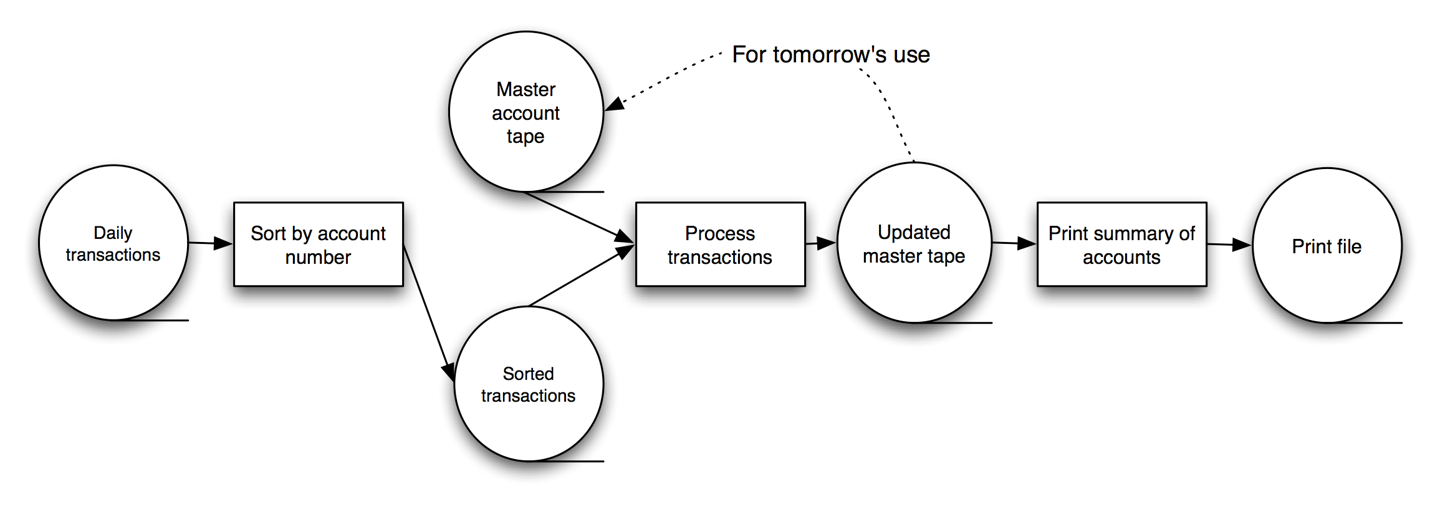
\includegraphics[width=0.7\textwidth]{batch.png}
			\attribution{N. Medvidovic}
		\end{center}
	\end{frame}

	\begin{frame}
		\frametitle{Пакетная обработка, Lunar Lander}
		\begin{center}
			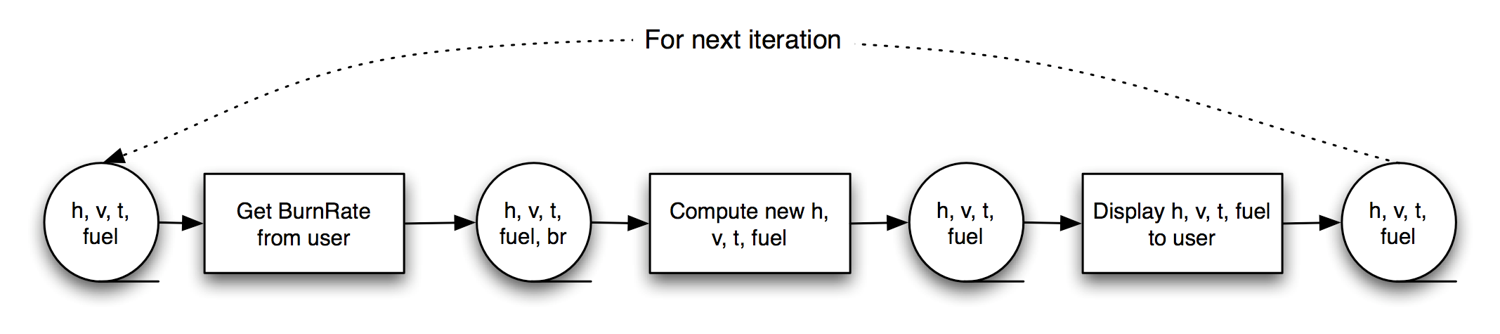
\includegraphics[width=0.95\textwidth]{batchLL.png}
			\attribution{N. Medvidovic}
		\end{center}
		Play-by-email?
	\end{frame}

	\section{Каналы и фильтры}

	\begin{frame}
		\frametitle{Каналы и фильтры}
		\framesubtitle{Pipes and filters}
		\begin{itemize}
			\item Компоненты --- это фильтры, преобразующие данные из входных каналов в данные в выходных каналах
			\item Соединители --- каналы
			\item Инварианты:
			\begin{itemize}
				\item Фильтры независимы (не имеют разделяемого состояния)
				\item Фильтры не знают о фильтрах до или после них
			\end{itemize}
			\item Вариации:
			\begin{itemize}
				\item Конвейеры --- линейные последовательности фильтров
				\item Ограниченные каналы --- где канал это очередь с ограниченным количеством элементов
				\item Типизированные каналы --- где каналы отличаются по типу передаваемых данных
			\end{itemize}
		\end{itemize}
	\end{frame}

	\begin{frame}
		\frametitle{Каналы и фильтры, подробности}
		\begin{itemize}
			\item Преимущества:
			\begin{itemize}
				\item Поведение системы --- это просто последовательное применение поведений компонентов
				\item Легко добавлять, заменять и переиспользовать фильтры
				\begin{itemize}
					\item Любые два фильтра можно использовать вместе
				\end{itemize}
				\item Широкие возможности для анализа
				\begin{itemize}
					\item Пропускная способность, задержки, deadlock-и
				\end{itemize}
				\item Широкие возможности для параллелизма
			\end{itemize}
			\item Недостатки:
			\begin{itemize}
				\item Последовательное исполнение
				\item Проблемы с интерактивными приложениями
				\item Пропускная способность определяется самым ``узким'' элементом
			\end{itemize}
		\end{itemize}
	\end{frame}

	\begin{frame}
		\frametitle{Каналы и фильтры, Lunar Lander}
		\begin{center}
			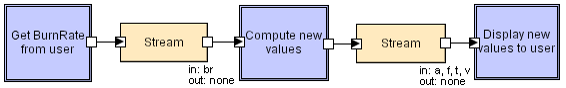
\includegraphics[width=0.85\textwidth]{pipesAndFiltersLL.png}
			\attribution{N. Medvidovic}
		\end{center}
	\end{frame}

	\section{Blackboard}

	\begin{frame}
		\frametitle{Blackboard}
		\begin{itemize}
			\item Два типа компонентов:
			\begin{itemize}
				\item Центральная структура данных --- та самая ``Blackboard''
				\item Компоненты, работающие с blackboard
			\end{itemize}
			\item Инварианты:
			\begin{itemize}
				\item Управление системой осуществляется только через состояние доски
				\item Компоненты не знают друг о друге и не имеют своего состояния
			\end{itemize}
			\item Часто применяется в системах искусственного интеллекта
		\end{itemize}
	\end{frame}

	\begin{frame}
		\frametitle{Blackboard, Lunar Lander}
		\begin{center}
			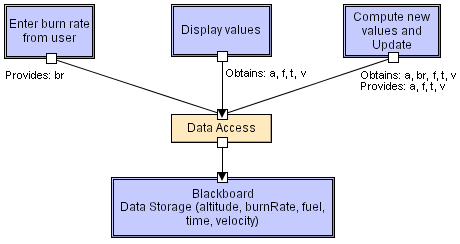
\includegraphics[width=0.6\textwidth]{blackboardLL.png}
			\attribution{N. Medvidovic}
		\end{center}
	\end{frame}

	\section{Стили с неявным вызовом}

	\begin{frame}
		\frametitle{Стили с неявным вызовом}
		\begin{itemize}
			\item Оповещение о событии вместо явного вызова метода
			\begin{itemize}
				\item ``Слушатели'' могут подписаться на событие
				\item Система при наступлении события сама вызывает все зарегистрированные методы слушателей
			\end{itemize}
			\item Компоненты имеют два вида интерфейсов --- методы и события
			\item Два типа соединителей:
			\begin{itemize}
				\item Явный вызов метода
				\item Неявный вызов по наступлению события
			\end{itemize}
			\item Инварианты:
			\begin{itemize}
				\item Те, кто производит события, не знают, кто и как на них отреагирует
				\item Не делается никаких предположений о том, как событие будет обработано и будет ли вообще
			\end{itemize}
		\end{itemize}
	\end{frame}

	\begin{frame}
		\frametitle{Стили с неявным вызовом, преимущества и недостатки}
		\begin{itemize}
			\item Преимущества:
			\begin{itemize}
				\item Переиспользование компонентов
				\begin{itemize}
					\item Очень низкая связность между компонентами
				\end{itemize}
				\item Лёгкость в конфигурировании системы
				\begin{itemize}
					\item Как во время компиляции, так и во время выполнения
				\end{itemize}
			\end{itemize}
			\item Недостатки:
			\begin{itemize}
				\item Зачастую неинтуитивная структура системы
				\item Компоненты не управляют последовательностью вычислений
				\item Непонятно, кто отреагирует на запрос и в каком порядке придут ответы
				\item Тяжело отлаживаться
				\item Гонки даже в однопоточном приложении
			\end{itemize}
		\end{itemize}
	\end{frame}

	\section{Publish-subscribe}

	\begin{frame}
		\frametitle{Издатель-подписчик}
		\framesubtitle{Publish-subscribe}
		\begin{itemize}
			\item Подписчики регистрируются, чтобы получать нужные им сообщения или данные. Издатели публикуют сообщения, синхронно или асинхронно.
			\item Компоненты: издатели, подписчики, ``маршрутизаторы''
			\item Соединители: как правило, сетевые протоколы, часто механизм наподобие паттерна ``Наблюдатель''
			\item Данные: подписки, нотификации, публикуемая информация
			\item Топология: подписчики подключаются к издателям напрямую, либо через посредников
			\item Преимущества: очень низкая связность между компонентами, при этом высокая эффективность распределения информации
		\end{itemize}
	\end{frame}

	\begin{frame}
		\frametitle{Издатель-подписчик, Lunar Lander}
		\begin{center}
			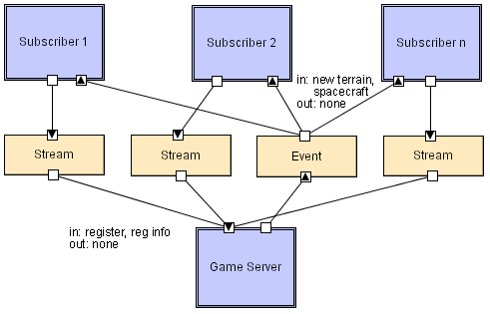
\includegraphics[width=0.6\textwidth]{pubSubLL.png}
			\attribution{N. Medvidovic}
		\end{center}
	\end{frame}

	\section{Событийно-ориентированный стиль}

	\begin{frame}
		\frametitle{Событийно-ориентированный стиль}
		\begin{itemize}
			\item Независимые компоненты посылают и принимают события, передаваемые по шинам
			\item Компоненты: независимые генераторы или потребители событий
			\item Соединители: шины событий (хотя бы одна)
			\item Данные: события и связаные с ними данные, посылаемые по шине
			\item Топология: компоненты общаются только с шинами событий, не друг с другом
			\item Варианты: push- и pull-режимы работы с шиной
			\item Преимущества: лёгкость масштабирования и добавления новой функциональности, эффективно для распределённых приложений
		\end{itemize}
	\end{frame}

	\begin{frame}
		\frametitle{Событийно-ориентированный Lunar Lander}
		\begin{center}
			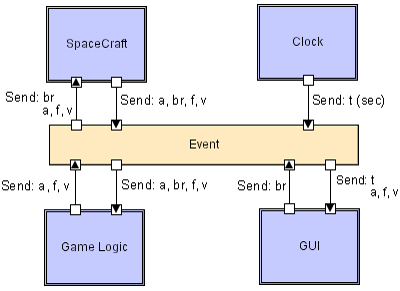
\includegraphics[width=0.45\textwidth]{eventBasedLL.png}
			\attribution{N. Medvidovic}
		\end{center}
	\end{frame}

	\section{Peer-to-peer}

	\begin{frame}
		\frametitle{Peer-to-peer}
		\begin{itemize}
			\item Состояние и поведение распределены между компонентами, которые могут выступать как клиенты и как серверы
			\item Компоненты: имеют своё состояние и свой поток управления
			\item Соединители: как правило, сетевые протоколы
			\item Элементы данных: сетевые сообщения
			\item Топология: сеть (возможно, с избыточными связями между компонентами), может динамически меняться
			\item Преимущества:
			\begin{itemize}
				\item Хорош для распределённых вычислений
				\item Устойчив к отказам
				\item Если протокол взаимодействия позволяет, легко масштабируется
			\end{itemize}
		\end{itemize}
	\end{frame}

	\begin{frame}
		\frametitle{Peer-to-peer Lunar Lander}
		\begin{center}
			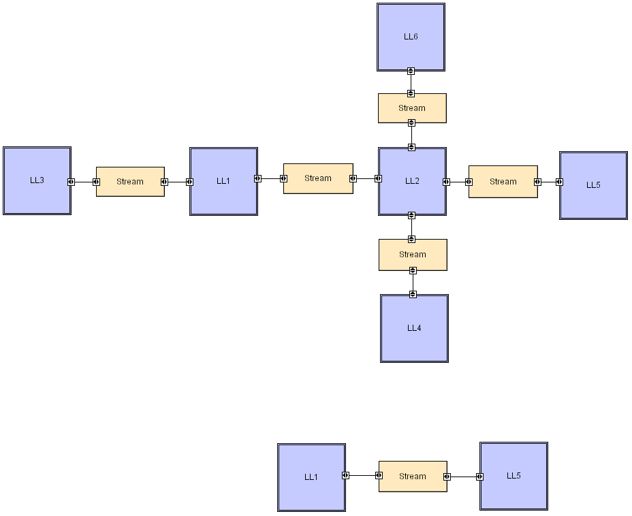
\includegraphics[width=0.7\textwidth]{peerToPeerLL.png}
			\attribution{N. Medvidovic}
		\end{center}
	\end{frame}

	\section{Гетерогенные стили}

	\begin{frame}
		\frametitle{Гетерогенные стили}
		\begin{itemize}
			\item Более сложные стили, полученные соединением простых стилей
			\begin{itemize}
				\item REST
				\item C2
				\item Распределённые объекты
				\begin{itemize}
					\item ОО + клиент-сервер
					\item CORBA
				\end{itemize}
			\end{itemize}
		\end{itemize}
	\end{frame}

	\section{C2}

	\begin{frame}
		\frametitle{C2}
		\begin{itemize}
			\item Стиль с неявным вызовом, где компоненты общаются только через коннекторы, маршрутизирующие сообщения
			\item Компоненты: независимые, потенциально параллельные производители или потребители
			\item Соединители: маршрутизаторы сообщений, которые могут фильтровать, преобразовывать и рассылать сообщения двух видов: нотификации и запросы
			\item Элементы данных: сообщения, содержащие данные
			\begin{itemize}
				\item Нотификации анонсируют изменения в состоянии
				\item Запросы --- запрашивают выполнение действия
			\end{itemize}
			\item Топология: слои компонентов и соединителей с определённым ``верхом'' и ``низом'', где нотификации шлются ``вниз'', а запросы --- ``вверх''
		\end{itemize}
	\end{frame}

	\begin{frame}
		\frametitle{С2 Lunar Lander}
		\begin{center}
			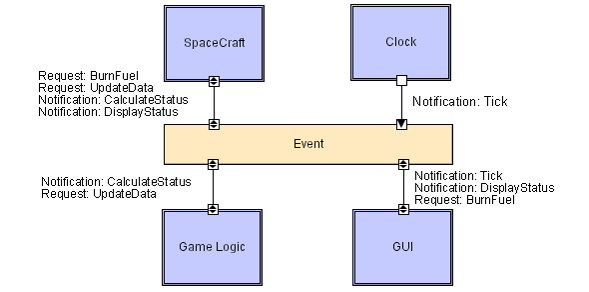
\includegraphics[width=0.6\textwidth]{c2LL.png}
			\attribution{N. Medvidovic}
		\end{center}
	\end{frame}

	\section{CORBA}

	\begin{frame}
		\frametitle{CORBA}
		\begin{itemize}
			\item ``Объекты'' работают на гетерогенных хостах, реализованные на разных языках программирования 
			\item Объекты предоставляют сервисы через чётко определённые интерфейсы и вызывают методы через RPC-протоколы
			\item Топология: граф объектов в самом общем смысле
			\item Дополнительные ограничения:
			\begin{itemize}
				\item Передаваемые при вызове метода данные должны быть сериализуемы
				\item Вызывающие должны обрабатывать ошибки, связанные с работой сети
			\end{itemize}
			\item Преимущества: независимость от платформы, языка и местоположения сервиса
		\end{itemize}
	\end{frame}

	\begin{frame}
		\frametitle{СORBA Lunar Lander}
		\begin{center}
			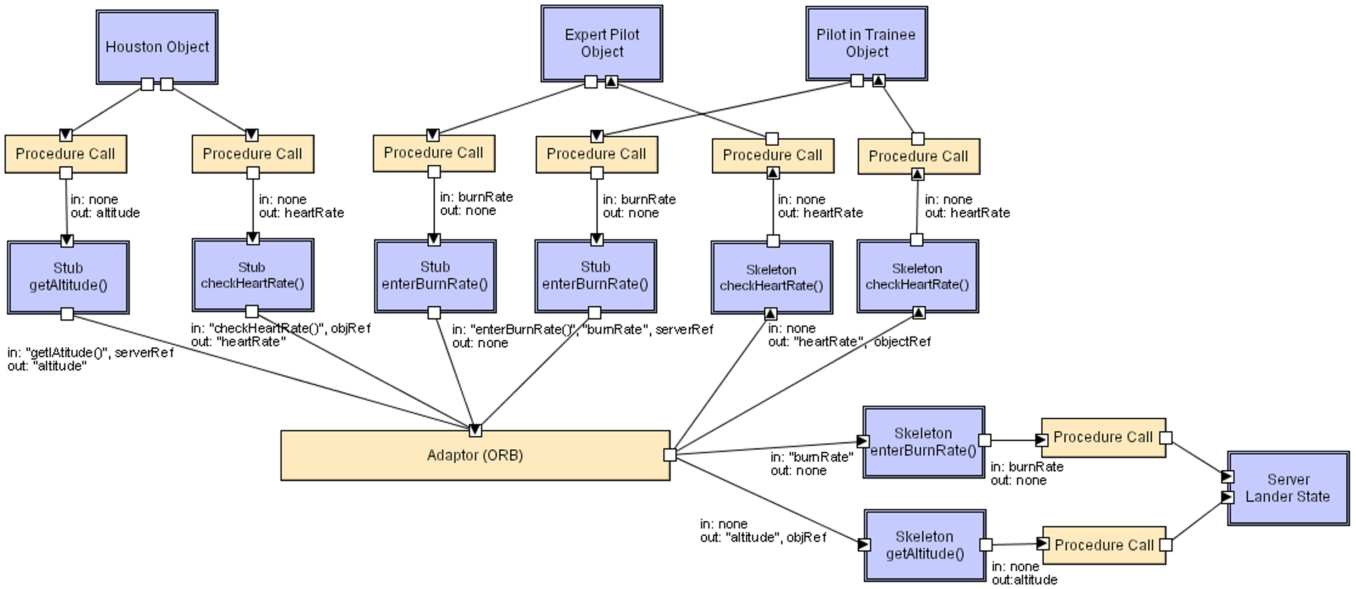
\includegraphics[width=0.9\textwidth]{corbaLL.png}
			\attribution{N. Medvidovic}
		\end{center}
	\end{frame}

\end{document}